\documentclass[10pt,a4paper]{article}

\usepackage[T1]{fontenc}
\usepackage[utf8]{inputenc}
\usepackage{newtxtext,newtxmath}
\usepackage[margin=1.9cm,top=1.6cm,bottom=1.8cm]{geometry}
\usepackage{graphicx,booktabs,tabularx,xcolor}
\usepackage[hidelinks]{hyperref}
\usepackage{titlesec,caption}

\definecolor{ink}{HTML}{16212E}
\definecolor{swissred}{HTML}{D52B1E}
\titleformat{\section}{\large\bfseries\color{ink}}{\thesection}{0.6em}{}
\titleformat{\subsection}{\normalsize\bfseries\color{ink}}{}{0pt}{}
\titlespacing*{\section}{0pt}{9pt}{4pt}
\titlespacing*{\subsection}{0pt}{7pt}{3pt}
\captionsetup{font=footnotesize,labelfont=bf,skip=4pt,hypcap=false}
\setlength{\parskip}{5pt}
\setlength{\parindent}{0pt}
\newcolumntype{L}{>{\raggedright\arraybackslash}X}
\hypersetup{pdftitle={The Neuron Migration},pdfauthor={Team NAMA}}

\begin{document}

\begin{minipage}{0.76\textwidth}
  {\LARGE\bfseries\color{ink} The Neuron Migration}\\[3pt]
  {\large Finding the rules behind the numbers}\\[6pt]
  {\bfseries Team NAMA}\\[2pt]
  Mohammad Javad Amin, Nava Biglar,\\
  Emad Aghajani, Maliheh Ghasemian\\[3pt]
  Neural Wave AI Hackathon 2026 \quad USI Lugano
\end{minipage}\hfill
\IfFileExists{../presentation/usi_logo.png}{\begin{minipage}{0.19\textwidth}\raggedleft
\includegraphics[width=\linewidth]{../presentation/usi_logo.png}\end{minipage}}{}

\section{Methodology}

Our approach was to use AI and statistical tools to investigate the data, then express the discovered rules as deterministic Python. The final calculations can be traced back to explicit decisions, while the tools help us decide which assumptions to test next.

\subsection{Establish what the records tell us}
We first connected policy information, transactions and historical changes to understand what was known at each point in time. We checked data inconsistencies before treating them as evidence of a calculation error. This distinction mattered, because an invalid date or inconsistent label could otherwise lead us to invent a rule that the system never used.

\subsection{Use discrepancies to choose the next hypothesis}
For each task, we started with the simplest rule and compared its output with the available targets. We grouped failures by policy characteristics and period, then asked what those cases had in common. Simple decision trees helped identify conditions associated with errors, and comparisons over time helped locate changes in behavior. We also compared alternative conventions when several explanations appeared plausible.

The aim was to explain a recurring pattern. A hypothesis became useful when it accounted for a group of failures and continued to work on the cases we already understood. We changed assumptions in controlled comparisons where possible, checked the consequences, and kept general rules rather than adding exceptions for individual policies.

\subsection{Check individual steps before the full history}
In fund accounting, one early error can affect every later balance. We therefore checked each calculation against the recorded state immediately before it. This allowed us to distinguish a wrong rule from a correct rule receiving an already incorrect balance.

We then replayed the complete sequence and compared the resulting outputs. Policy values, annual statements and taxes shared the same accounting foundation, so a change in one place could be checked against related tasks. Exact monetary comparisons were essential since a close result could still reveal the wrong convention.

\subsection{Treat historical changes as part of the rules}
A major turning point was recognizing the effect of the 2007 system conversion. A single convention did not explain both periods. For example, older payment schedules could retain a date shift caused by a short month, while the newer system returned to an anchored schedule.

We used this distinction to guide the rest of the investigation. Dates, changing terms and operational timing became part of the explanation, rather than background information. The same discovery process could then be reused across tasks: identify the pattern, propose a rule and check it against the available evidence.

\subsection{Approach to t7: working with limited evidence}
The surprise tax task (``t7'') was harder because target data was (initially) unavailable. Without direct comparisons, our early investigation was more speculative: we considered, for example, whether tax calculations varied by canton as well as by country. Tax-booking records, worked examples and consistency checks helped narrow the possibilities, but could not settle every assumption. Samples released later by the organisers allowed us to test these ideas more directly.

\newpage
\section{Results}

On the 3,019 training policies, the supplied local scorer gave the following exact-match results:

\vspace{3pt}
\begin{minipage}[t]{0.51\textwidth}
\vspace{0pt}
\begin{tabularx}{\linewidth}{@{}Lr@{}}
\toprule
Task & Accuracy \\
\midrule
Commission & 99.996\,\% \\
Next due dates & 100\,\% \\
Projected maturity value & 99.735\,\% \\
Surrender value & 99.740\,\% \\
Annual statement & 99.939\,\% \\
\bottomrule
\end{tabularx}
\end{minipage}\hfill
\begin{minipage}[t]{0.44\textwidth}
\vspace{0pt}
Outlier analysis identified 55 remaining discrepancies: 38 documented manual corrections and 17 additional suspected edits. We kept these visible rather than adding exceptions to match individual targets. These are training results, not estimates for unseen policies.
\end{minipage}
\vspace{3pt}

\subsection{Historical rules remove a persistent error pattern}
Applying only the newer conventions produces substantial errors for older policies (Figure~\ref{fig:eras}). Statement errors persist after conversion because later balances inherit earlier differences. Reconstructing the historical rules removes this systematic pattern.

\begin{center}
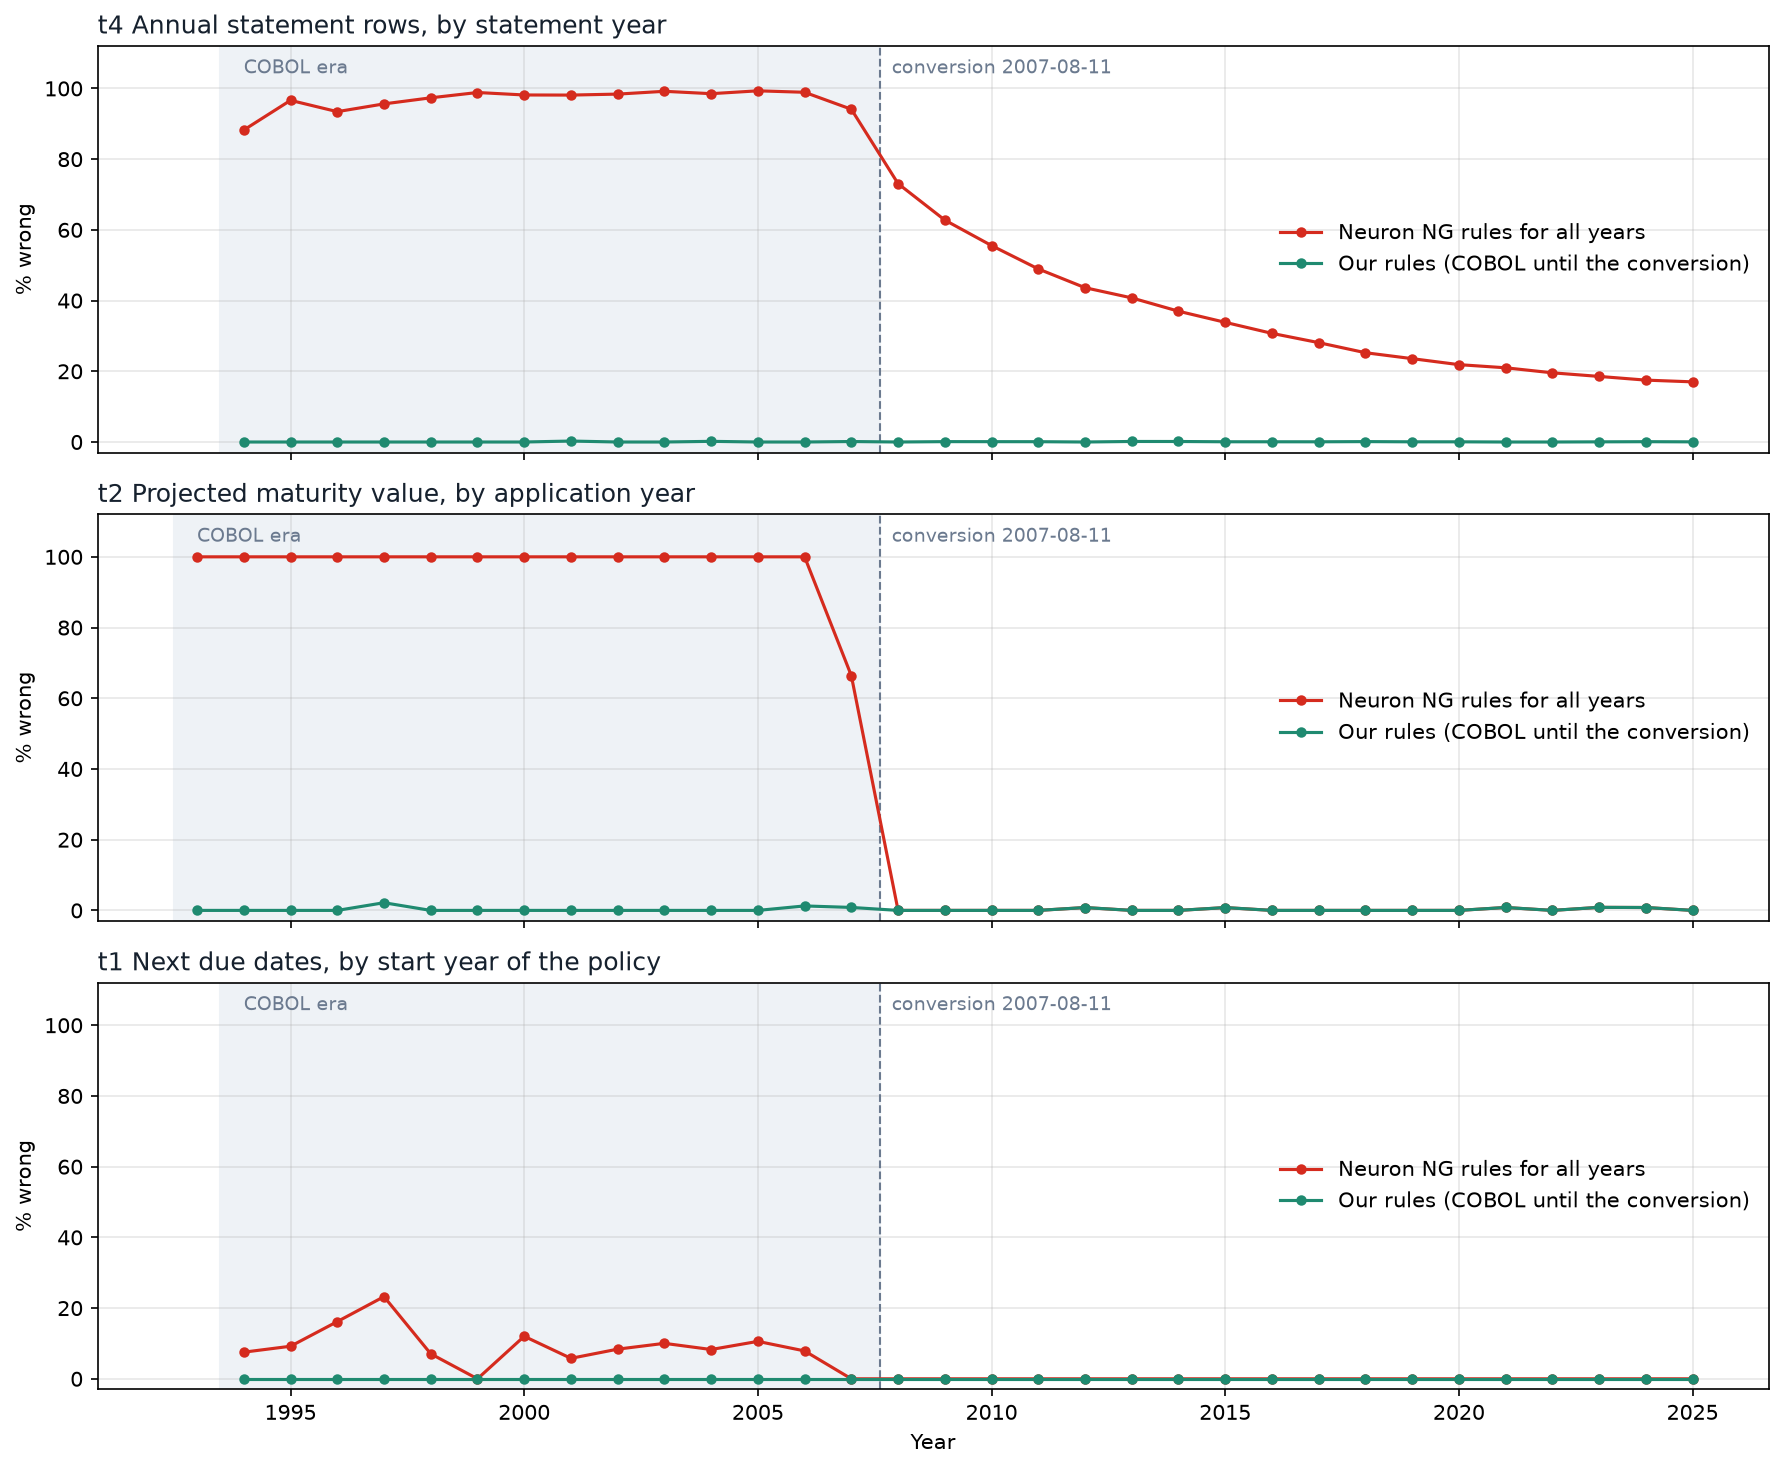
\includegraphics[width=0.86\textwidth]{../Plots/errors_by_era.png}
\captionof{figure}{Incorrect outputs by year for annual statements, maturity projections and due dates. Red applies the newer rules throughout; green uses the reconstructed historical rules. Shading marks the older system period.}
\label{fig:eras}
\end{center}

\subsection{t7 results and limitations}
Local checks against the two released tax samples gave the following results:

\begin{center}
\begin{tabular}{@{}lrr@{}}
\toprule
Released sample & Exact payouts & Exact annual rows \\
\midrule
Sample 1 & 19 / 20 & 20 / 20 \\
Sample 2 & 40 / 40 & 30 / 30 \\
\bottomrule
\end{tabular}
\end{center}

These samples were used during development. The latest recorded leaderboard result was lower: 10/40 payouts and 29/30 annual rows. The difference remains unresolved, and one released payout still differs locally by a cent. We report these outcomes separately rather than treating the sample matches as independent validation.

\newpage
\section{Challenges}

\subsection{Reading patterns without overinterpreting them}
The tax timeline provided evidence beyond target values. Changes in booking frequency and processing times helped us select periods for closer investigation. The shift around 2007 is visible in the middle panel; the bottom panel shows same-day recording for the plotted payout bookings. These observations constrained our hypotheses without establishing the tax formulas themselves.

\begin{center}
% Cached rendering of the timeline; the original JPEG is currently unreadable.
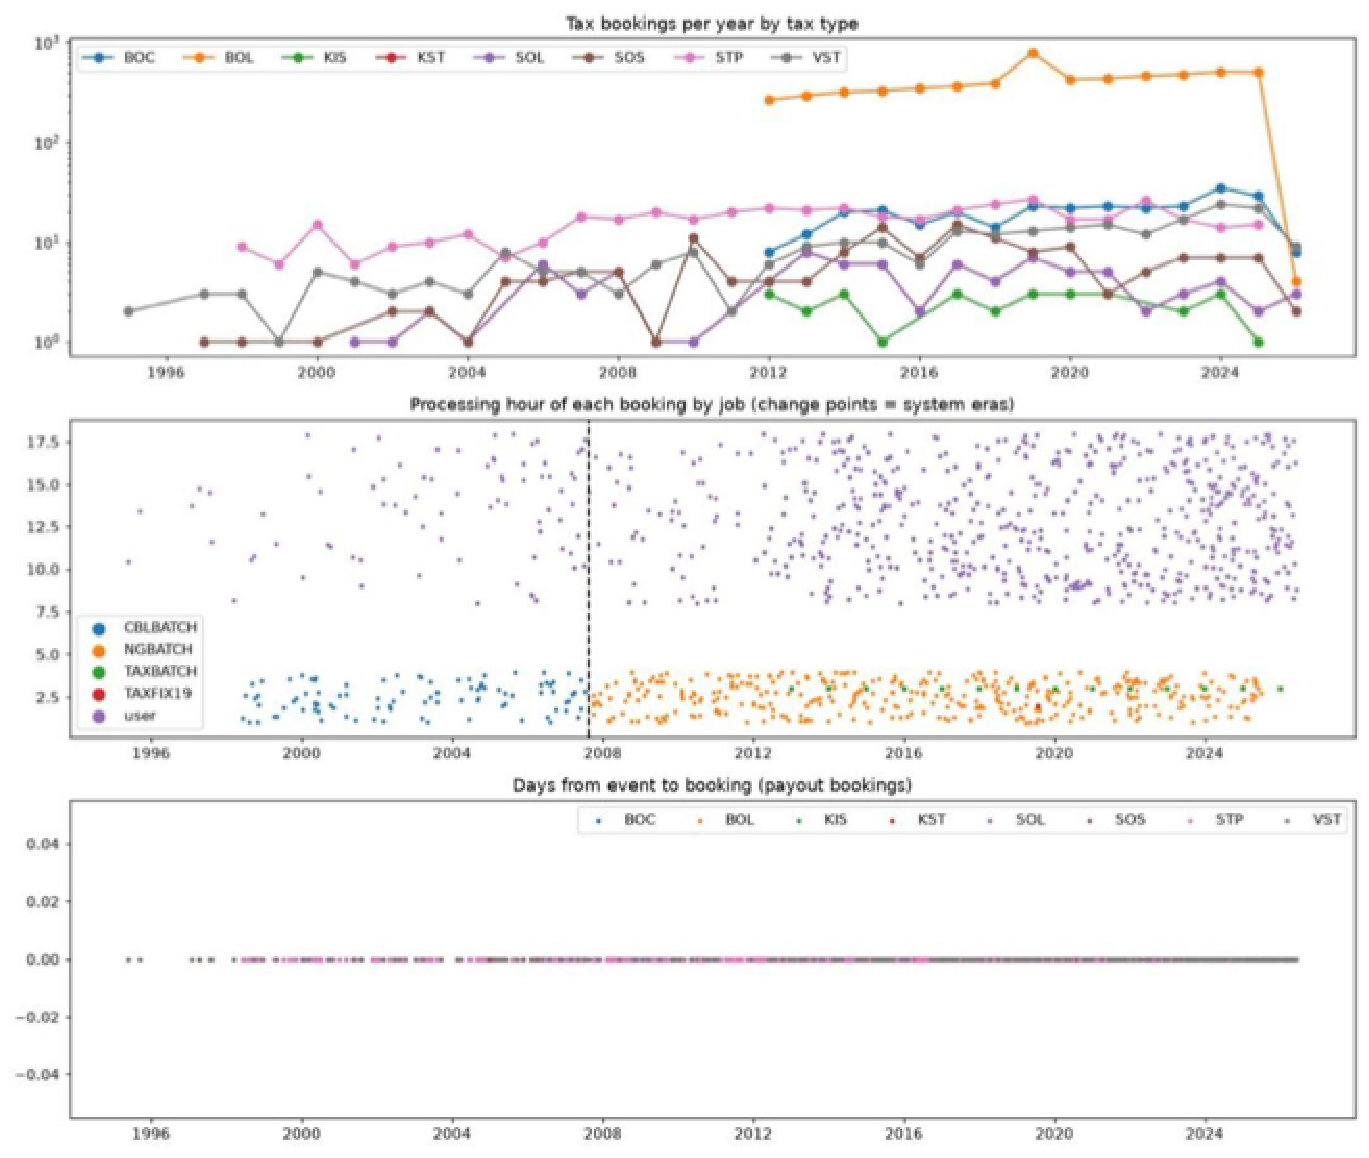
\includegraphics[width=0.90\textwidth]{tax_timeline_preview.pdf}
\captionof{figure}{Tax-booking timeline: annual counts by tax type (top), processing hour by job (middle), and days between payout events and bookings (bottom). The dashed line marks the system transition.}
\label{fig:timeline}
\end{center}

\subsection{What did not work}
Applying the newer conventions to all periods failed on older policies. Familiar financial and legal conventions also proved insufficient without direct checks. Early comparisons were too tolerant and hid small monetary errors; exact comparisons exposed the remaining differences.

Aggregate tax scores were difficult to interpret because several fields could be wrong in the same row. Fixing one field might leave the score unchanged. Released examples made the investigation more focused, but also increased the risk of fitting too closely to known cases. Broader tax accuracy remains an open question.

\section{Takeaways}
The same discovery process can be reused across tasks: investigate recurring discrepancies, test explanations and turn supported rules into explicit code. Reconstructing historical behavior makes that code reflect how the system actually evolved.

\end{document}
